\section{Аппаратные возможности потока управления}
\label{sec:Goto}

В скалярных архитектурах поток управления обычно реализован через инструкции
условных переходов. При этом условие, от которого зависит переход, всегда также
является скалярным. В отличие от этого в векторной модели может возникать
векторное условие, верное для одних линий исполнения и неверное для других.
В архитектурах не поддерживающих векторный поток управления такой случай может
быть сведен к скалярному путем маскированного исполнения всех инструкций дуги
условного перехода или как минимум маскированного исполнения инструкций этой
дуги, имеющих побочные эффекты (обычно это только записи в память).

В графических ускорителях Intel есть возможность использовать векторный поток
управления без сведения его к скалярному случаю. Это реализовано через две
команды: \texttt{goto} и \texttt{join}. Особенностью команды \texttt{goto}
является возможность ее предикатирования. В этом случае исполнение программы
произойдет так, что для предикатированных элементов вектора произойдет переход
по указанной метке, а для всех остальных элементов произойдет переход на
следующую инструкцию. Команда \texttt{join} синхронизирует исполнение
инструкций.

В аппаратуре подобная модель исполнения реализуется с помощью маски исполнения
(\textit{англ. execution mask}). Каждый бит этой маски соответствует элементу
вектора. Если бит установлен в 0, то для соответствующего элемента вычисления не
производятся, если же бит установлен в 1, то для соответствующего элемента
исполнение происходит в обычном режиме. В самом начале программы маска состоит
из единиц. Изменения в маске производят инструкции \texttt{goto} и \texttt{join}.
Команда \texttt{goto} устанавливает в соответствии с предикатом биты маски в 0,
выключая линии вектора, для которых условие не выполняется. Команда \texttt{join}
восстанавливает маску до того состояния, в котором она находилась до изменения
соответствующим \texttt{goto}.

Рассмотрим пример кода с векторным потоком управления на языке ассемблера для
архитектуры графических ускорителей Intel. В данном примере реализована
высокоуровневая конструкция if-else. Если элемент выбранного вектора
\texttt{r2.0<8;8,1>:d} больше или равен нулю, то в вектор \texttt{r3.0<1>:d} он
будет записан увеличенным на 1, в противном случае - уменьшенным на 1.

\begin{verbatim}
...
(W)     cmp  (8|M0) (gt)f0.0 null<1>:d r2.0<8;8,1>:d -1:w
(~f0.0) goto (8|M0)          BB_2      BB_2
BB_1:
(W)     add  (8|M0)          r3.0<1>:d r2.0<8;8,1>:d  1:w
(f0.0)  goto (8|M0)          BB_2      BB_4
BB_2:
        join (8|M0)          BB_2
BB_3:
        add  (8|M0)          r3.0<1>:d r2.0<8;8,1>:d -1:w
BB_4:
        join (8|M0)          BB_2
BB_5:
...
\end{verbatim}

\begin{figure}[h]
  \centering
  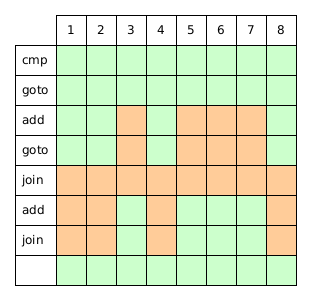
\includegraphics[scale=0.60]{Images/HW-goto-example.png}
  \caption{Схема исполнения представленного примера с векторным потоком
  управления}
  \label{fig:HW-goto-example}
\end{figure}

На рисунке ~\ref{fig:HW-goto-example} схематично изображено, как будет
происходить исполнение данного кода. Цифрами сверху обозначены номера линий
исполнения в SIMD-8 АЛУ, зеленым обозначены включенные линии, а оранжевым -
выключенные.
